\documentclass[aspectratio=169,10pt]{beamer}

\usepackage[T1]{fontenc}
\usepackage[utf8]{inputenc}
\usepackage[brazilian,provide=*]{babel}
\usepackage{lmodern}
\usepackage{textcomp}
\usepackage{booktabs}
\usepackage{array}
\usepackage{listings}
\usepackage{tikz}
\usetikzlibrary{positioning,arrows.meta,fit}

% ---------- estilo: minimalista, preto e cinza ----------
\usefonttheme{serif}
\setbeamersize{text margin left=7mm, text margin right=7mm}
\setbeamertemplate{navigation symbols}{}
\setbeamercolor{structure}{fg=black}
\setbeamercolor{normal text}{fg=black}
\setbeamercolor{frametitle}{fg=black}
\setbeamercolor{title}{fg=black}
\setbeamerfont{frametitle}{size=\large,series=\bfseries}
\setbeamertemplate{itemize item}{\color{black!55}\raisebox{0.15ex}{\scriptsize$\blacksquare$}}
\setbeamertemplate{itemize subitem}{\color{black!45}--}
\setbeamertemplate{footline}{\hfill\color{black!45}\scriptsize\insertframenumber\hspace{1.2em}\vspace{0.8em}}
\setlength{\leftmargini}{1.1em}

\definecolor{cinza}{gray}{0.42}

% ---------- código: cópia literal dos arquivos do trabalho ----------
% Os trechos em trechos/ são gerados por extrai_trechos.py a partir de
% trabalho_final_ferr_comp.R, 03_verificacao.sql e dos blocos P1 a P4.
\lstdefinestyle{codigo}{
  basicstyle=\ttfamily\fontsize{6.5}{7.9}\selectfont,
  columns=fullflexible, keepspaces=true, showstringspaces=false,
  upquote=true, breaklines=true, breakatwhitespace=true,
  frame=leftline, framerule=0.6pt, rulecolor=\color{black!30},
  xleftmargin=0.8em, aboveskip=0.3em, belowskip=0.3em,
  morecomment=[l]{\#}, morestring=[b]", commentstyle=\color{cinza},
  literate={á}{{\'a}}1 {ã}{{\~a}}1 {ê}{{\^e}}1 {í}{{\'i}}1 {ó}{{\'o}}1
           {ú}{{\'u}}1 {Ê}{{\^E}}1 {é}{{\'e}}1 {ç}{{\c{c}}}1 {õ}{{\~o}}1
           {â}{{\^a}}1 {à}{{\`a}}1 {Í}{{\'I}}1 {~}{{\texttildelow}}1}
\lstdefinestyle{codigomenor}{style=codigo,
  basicstyle=\ttfamily\fontsize{6}{7.3}\selectfont}
\lstdefinestyle{codigomaior}{style=codigo,
  basicstyle=\ttfamily\fontsize{7.6}{9.3}\selectfont}
\lstdefinestyle{codigomedio}{style=codigo,
  basicstyle=\ttfamily\fontsize{7}{8.5}\selectfont}
\lstdefinestyle{codigosql}{style=codigo, morecomment=[l]{--}}

\newcommand{\trecho}[2][codigo]{\lstinputlisting[style=#1]{trechos/#2}}
\newcommand{\fonte}[1]{{\scriptsize\color{cinza}#1}}
\newcommand{\cab}[1]{{\small\bfseries #1}\par\vspace{0.3em}}
\newcommand{\cod}[1]{\texttt{#1}}

\title{Uma base de dados relacional da pós-graduação brasileira}
\subtitle{Astronomia/Física e Química nos dados abertos da CAPES (2021--2024)}
\author{Fernando Casellato \quad Felipe Piancatelli\\[0.2em] Ana Carolina Soares \quad Marcos Antônio Garcia}
\institute{Ferramentas Computacionais \\ Docente: Thomas Nogueira Vilches}
\date{}

\begin{document}

% ====================================================================== P2.1
\begin{frame}{P2 $\cdot$ Consulta}
  \begin{columns}[T]
    \column{0.64\textwidth}
    \trecho[codigomenor]{p2_consulta.R}
    \vspace{0.4em}
    \trecho[codigomenor]{p2_prog.R}
    \column{0.32\textwidth}
    \small
    \begin{itemize}
      \item \cod{DISTINCT ON}: cada docente conta uma vez por área e ano, no programa de nota mais alta
      \item Os programas novos (conceito A) ficam de fora
      \item \cod{nivel\_pq}: nível 1 (1A a 1D e sênior), nível 2 ou sem bolsa
      \item \cod{summarise}: uma linha por programa, com docentes e bolsistas
    \end{itemize}
  \end{columns}
\end{frame}

% ====================================================================== P2.1b
\begin{frame}{P2 $\cdot$ Modelo}
  \begin{columns}[T]
    \column{0.64\textwidth}
    \trecho[codigomaior]{p2_modelo.R}
    \vspace{0.6em}
    \trecho[codigomaior]{p2_interacao.R}
    \column{0.32\textwidth}
    \small
    \begin{itemize}
      \item \cod{cbind}: a resposta são os bolsistas e os não bolsistas de cada programa
      \item \cod{relevel}: a nota 4 é a referência
      \item \cod{quasibinomial}: erros-padrão corrigidos pela variação entre programas
      \item \cod{anova} com teste F: o efeito da nota é o mesmo nas duas áreas?
    \end{itemize}
  \end{columns}
\end{frame}

% ====================================================================== P2.2
\begin{frame}{P2 $\cdot$ Gráfico por programa}
  \begin{columns}[T]
    \column{0.64\textwidth}
    \trecho[codigomedio]{p2_ggplot.R}
    \column{0.32\textwidth}
    \small
    \begin{itemize}
      \item \cod{geom\_point}: um ponto por programa, com deslocamento lateral para não sobrepor
      \item \cod{geom\_errorbar} com \cod{ymin = ymax}: um traço no percentual do conjunto de docentes da área e da nota
      \item \cod{cores\_area}: cada área tem a mesma cor em todos os gráficos
    \end{itemize}
  \end{columns}
\end{frame}

% ====================================================================== P2.3
\begin{frame}{P2 $\cdot$ Bolsistas de produtividade por nota do programa}
  \begin{columns}[c]
    \column{0.63\textwidth}
    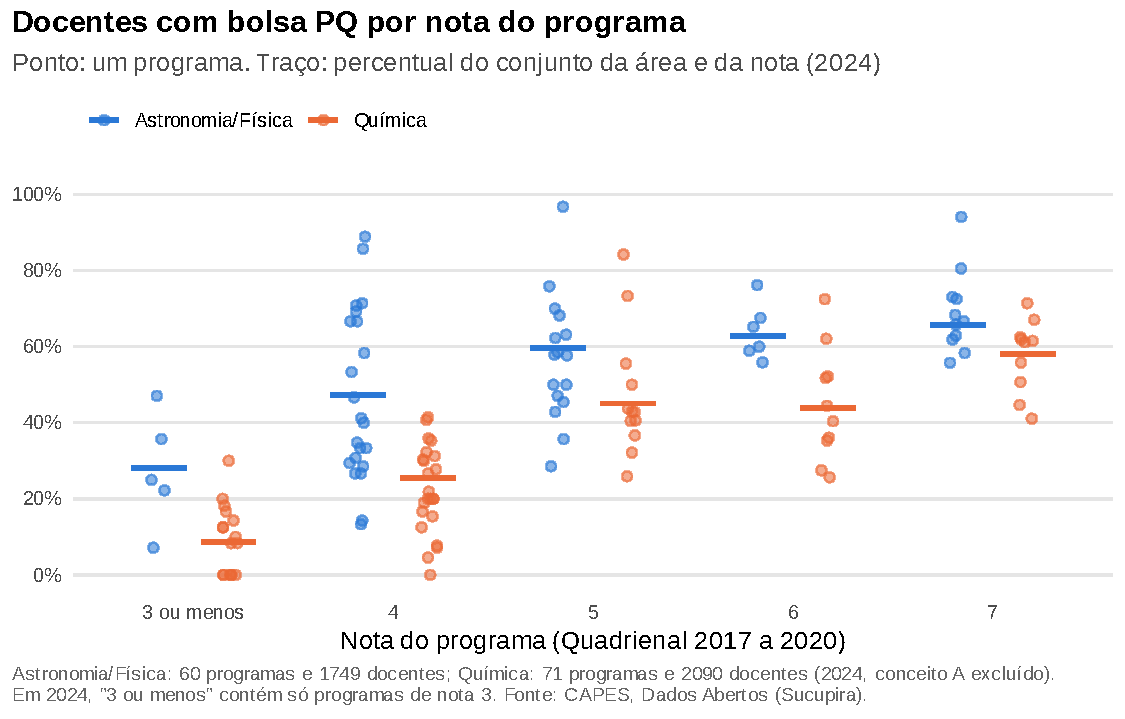
\includegraphics[width=\linewidth]{figuras_v2/P2_pq_por_nota_programas.pdf}
    \column{0.34\textwidth}
    \small
    \begin{itemize}
      \item 2024: 58,0\% dos docentes de Astronomia/Física e 39,4\% dos de Química têm bolsa
      \item Da nota 3 à nota 7: de 28\% a 66\% e de 9\% a 58\%
      \item Entre os programas: de 7\% a 97\% e de 0\% a 84\%
      \item Programas de mesma área e mesma nota diferem em dezenas de pontos percentuais
    \end{itemize}
  \end{columns}
\end{frame}

% ====================================================================== P2.4
\begin{frame}{P2 $\cdot$ Regressão logística sobre os programas}
  \begin{columns}[T]
    \column{0.50\textwidth}
    \small
    \begin{tabular}{@{}lcc@{}}
      \toprule
      termo & razão de chances & IC 95\% \\
      \midrule
      Química & 0,52 & 0,42 a 0,64 \\
      nota 3  & 0,33 & 0,19 a 0,58 \\
      nota 5  & 2,00 & 1,48 a 2,69 \\
      nota 6  & 2,06 & 1,49 a 2,84 \\
      nota 7  & 3,00 & 2,28 a 3,94 \\
      \bottomrule
    \end{tabular}

    \vspace{0.6em}
    \fonte{Referência: Astronomia/Física, nota 4. 131 programas e 3839 docentes.\\
           Dispersão estimada: 2,32.}
    \column{0.46\textwidth}
    \small
    \begin{itemize}
      \item Nota como tendência linear: razão de chances de 1,49 por ponto (IC 95\% de 1,37 a 1,61)
      \item Notas 5 e 6 têm razões quase iguais
      \item Interação área $\times$ nota: $p = 0{,}10$ com a nota em categorias e $p = 0{,}006$ com a nota como tendência
      \item Tendência em cada área: 1,31 por ponto em Astronomia/Física e 1,65 em Química
    \end{itemize}
  \end{columns}
\end{frame}

% ====================================================================== P2.5
\begin{frame}{P2 $\cdot$ Gráficos do nível da bolsa e da evolução}
  \begin{columns}[T]
    \column{0.64\textwidth}
    \trecho[codigomenor]{p2_comp.R}
    \trecho[codigomenor]{p2_evolucao.R}
    \column{0.32\textwidth}
    \small
    \begin{itemize}
      \item \cod{count} e \cod{group\_by}: percentual de cada nível dentro de cada área e nota
      \item \cod{geom\_col}: barras de 100\%, uma por nota, com um painel por área
      \item A evolução usa todos os anos da consulta, não só 2024
      \item \cod{geom\_text} no último ano escreve o nome da área e dispensa a legenda
    \end{itemize}
  \end{columns}
\end{frame}

% ====================================================================== P2.6
\begin{frame}{P2 $\cdot$ Nível da bolsa por nota do programa}
  \begin{columns}[c]
    \column{0.60\textwidth}
    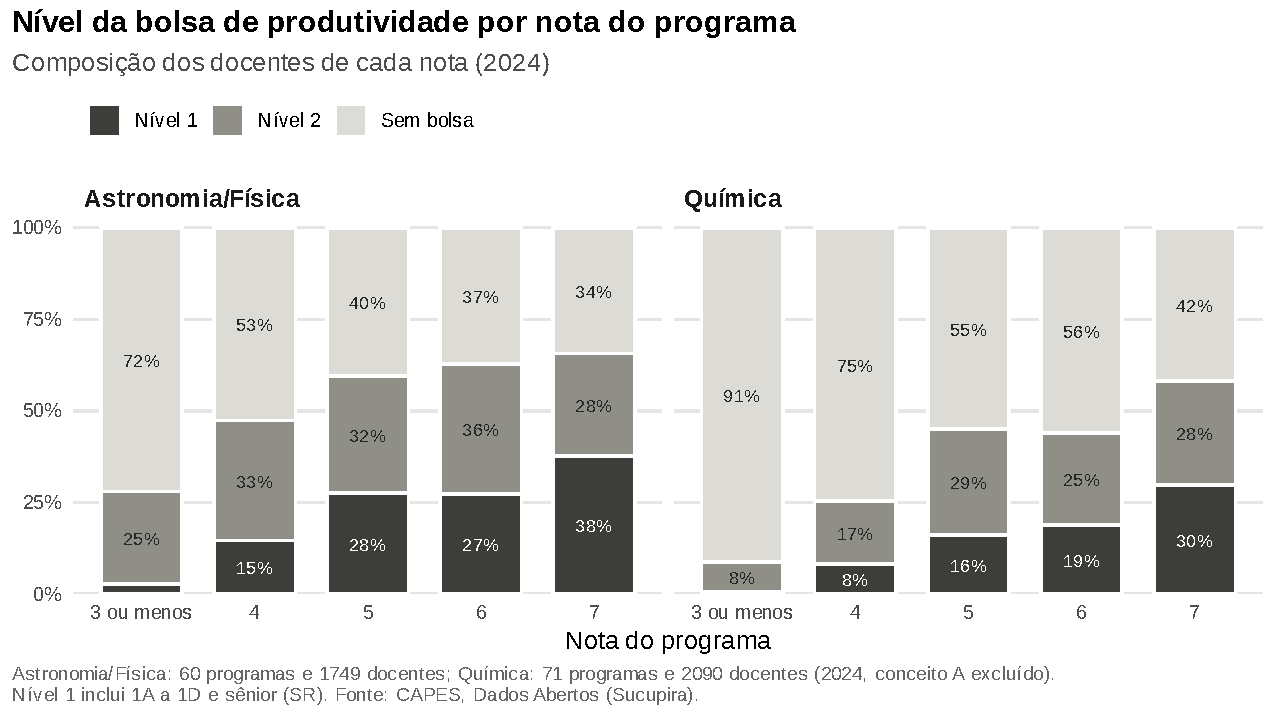
\includegraphics[width=\linewidth]{figuras_v2/P2_nivel_pq_por_nota.pdf}
    \column{0.37\textwidth}
    \small
    \begin{itemize}
      \item Em 2024: nível 1, nível 2 e sem bolsa são 27\%, 31\% e 42\% dos docentes de Astronomia/Física e 17\%, 23\% e 61\% dos de Química
      \item Nível 1 (1A a 1D e sênior): de 15\% na nota 4 a 38\% na nota 7 em Astronomia/Física, e de 8\% a 30\% na Química
      \item Na nota 3 ou menos há 2 docentes de nível 1 em Astronomia/Física e 1 na Química
    \end{itemize}
  \end{columns}
\end{frame}

% ====================================================================== P2.7
\begin{frame}{P2 $\cdot$ Bolsistas de produtividade de 2021 a 2024}
  \begin{columns}[c]
    \column{0.60\textwidth}
    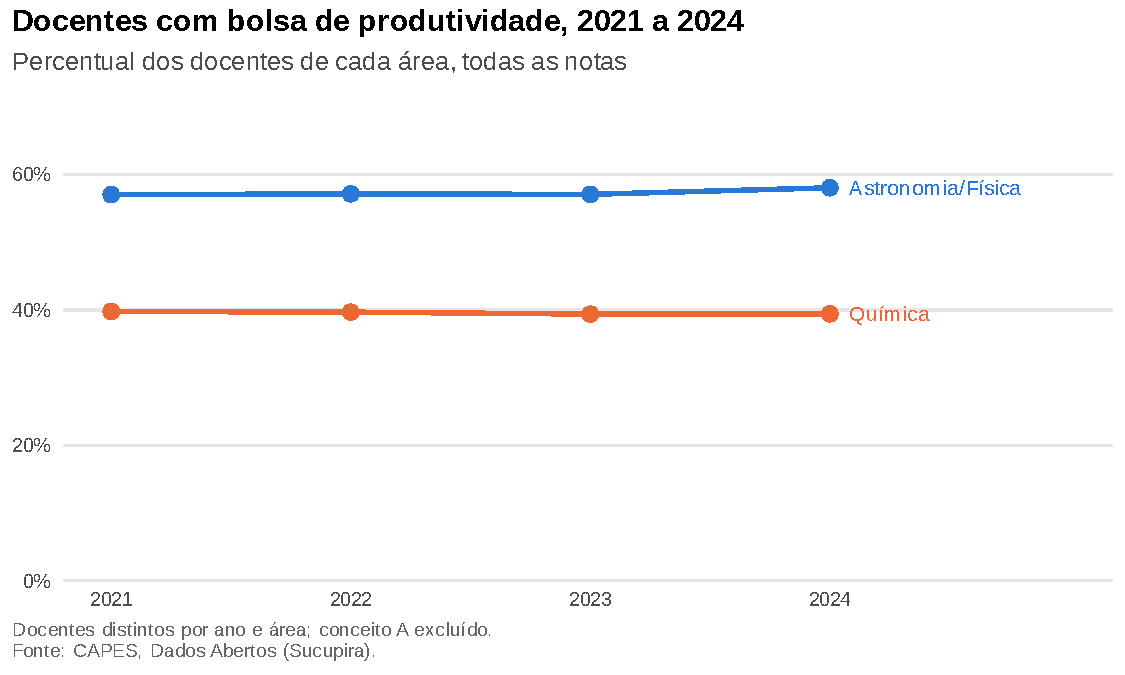
\includegraphics[width=\linewidth]{figuras_v2/P2_evolucao_pq.pdf}
    \column{0.37\textwidth}
    \small
    \begin{itemize}
      \item Astronomia/Física: 57,0\% em 2021 (990 de 1736) e 58,0\% em 2024 (1015 de 1749)
      \item Química: 39,8\% em 2021 (851 de 2139) e 39,4\% em 2024 (824 de 2090)
      \item Em quatro anos os percentuais variam cerca de 1 ponto em Astronomia/Física e menos de 0,5 ponto na Química
      \item Docentes distintos por ano e área, sem os programas de conceito A
    \end{itemize}
  \end{columns}
\end{frame}

% ====================================================================== P2.8
\begin{frame}{Síntese da P2}
  \begin{columns}[T]
    \column{0.47\textwidth}
    \cab{Os dados mostram}
    \begin{itemize}
      \item Em programas de mesma nota, a bolsa de produtividade é menos frequente na Química (razão de chances 0,52)
      \item A proporção de bolsistas cresce com a nota nas duas áreas, e a de bolsistas de nível 1 também
      \item De 2021 a 2024 os percentuais ficaram entre 57\% e 58\% em Astronomia/Física e entre 39\% e 40\% na Química
    \end{itemize}
    \column{0.47\textwidth}
    \cab{Os dados não permitem afirmar}
    \begin{itemize}
      \item Que a nota atraia bolsas ou que as bolsas elevem a nota: a Quadrienal 2017--2020 avaliou em parte a produção desses mesmos docentes
      \item Que a diferença entre as áreas meça desempenho: as bolsas são distribuídas por área no CNPq
      \item Que o aumento com a nota seja mais forte na Química: o resultado muda com a forma de incluir a nota no modelo
    \end{itemize}
  \end{columns}
\end{frame}

\end{document}
